\documentclass[submit]{harvardml}

% Put in your full name and email address.
\name{Melissa Yu}
\email{melissayu@college.harvard.edu}

% List any people you worked with.
\collaborators{%
  Alex Lin
}

% You don't need to change these.
\course{CS281-F17}
\assignment{Assignment \#1 v 1.2}
\duedate{5:00pm September 22, 2017}

\usepackage{url, enumitem}
\usepackage{amsfonts}
\usepackage{listings}
\usepackage{bm}
\usepackage{hyperref}
\usepackage[OT1]{fontenc}
\usepackage[pdftex]{graphicx}

% Some useful macros.
\newcommand{\given}{\,|\,}
\newcommand{\R}{\mathbb{R}}
\newcommand{\E}{\mathbb{E}}
\newcommand{\var}{\text{var}}
\newcommand{\cov}{\text{cov}}
\newcommand{\N}{\mathcal{N}}
\newcommand{\ep}{\varepsilon}

\newcommand{\Dir}{\text{Dirichlet}}
\newcommand{\norm}[1]{\left\lVert#1\right\rVert}
\newcommand\independent{\protect\mathpalette{\protect\independenT}{\perp}}

\begin{document}

%%%%%%%%%%%%%%%%%%%%%%%%%%%%%%%%%%%%%%%%%%%%%%%%%%%%%%%%
%%%%%%%%%%%%%%%%% PROBLEM 1 %%%%%%%%%%%%%%%%%%%%%%%%%%%%
%%%%%%%%%%%%%%%%%%%%%%%%%%%%%%%%%%%%%%%%%%%%%%%%%%%%%%%%
\begin{problem}[A Classic on the Gaussian Algebra, 10pts]
  Let $X$ and $Y$ be independent univariate Gaussian random
 variables. In the previous problem set, you likely used the closure property that $Z = X + Y$ is also a Gaussian random variable. Here you'll prove this fact.

\begin{enumerate}[label=(\alph*)]
\item Suppose $X$ and $Y$ have mean 0 and variances $\sigma_X^2$ and $\sigma_Y^2$ respectively. Write the pdf of $X + Y$ as an integral.
\item Evaluate the integral from the previous part to find a closed-form expression for the pdf of $X+Y$, then argue that this expression implies that $X+Y$ is also Gaussian with mean $0$ and variance $\sigma_X^2 + \sigma_Y^2$. Hint: what is the integral, over the entire real line, of
\[
f(x) = \frac{1}{\sqrt{2\pi}\sigma} \exp\left( -\frac{1}{2\sigma^2}(x - \mu)^2 \right) ,
\] i.e., the pdf of a univariate Gaussian random variable?
\item Extend the above result to the case in which $X$ and $Y$ may have arbitrary means.
\item Univariate Gaussians are supported on the entire real line. Sometimes this is undesirable because we are modeling a quantity with positive support. A common way to transform a Gaussian to solve this problem is to exponentiate it. Suppose $X$ is a univariate Gaussian with mean $\mu$ and variance $\sigma^2$. What is the pdf of $e^X$?
\end{enumerate}
\vspace{0.1cm}
\end{problem}

\begin{enumerate}[label=(\alph*)]
	\item Let $f_X(x)$ and $f_Y(y)$ be the pdfs of $X$ and $Y$, respectively. Then, we can express the pdf of $Z$ as the marginalization of the joint pdf $(Z, Y)$. We have
	\begin{align*}
	f_Z(z) &= \int_{-\infty}^{\infty} f_X(z - y) f_Y(y) dy \\
	&= \int_{-\infty}^{\infty} \frac{1}{2\pi\sigma_X\sigma_Y} \exp\left[ -\frac{1}{2}\left(\frac{(z - y)^2}{\sigma_X^2} + \frac{y^2}{\sigma_Y^2}\right) \right] dy
	\end{align*}
	
	\item We complete the square in the exponent to get
	\begin{align*}
	\frac{(z - y)^2}{\sigma_X^2} + \frac{y^2}{\sigma_Y^2} 
	&= \frac{1}{\sigma_X^2\sigma_Y^2}\left[(\sigma_X^2 + \sigma_Y^2) (y - \frac{\sigma_Y^2}{\sigma_X^2 + \sigma_Y^2} z)^2 + \frac{\sigma_X^2\sigma_Y^2}{\sigma_X^2 + \sigma_Y^2} z^2\right] \\
	&= \frac{\sigma_X^2 + \sigma_Y^2}{\sigma_X^2\sigma_Y^2} (y - \frac{\sigma_Y^2}{\sigma_X^2 + \sigma_Y^2} z)^2 + \frac{1}{\sigma_X^2 + \sigma_Y^2} z^2 \\
	&= \frac{1}{\sigma^2} (y - \mu)^2 + \frac{1}{\sigma_X^2 + \sigma_Y^2} z^2,
	\end{align*}
	where $\sigma = \frac{\sigma_X\sigma_Y}{\sqrt{\sigma_X^2 + \sigma_Y^2}}$ and $\mu = \frac{\sigma_Y^2}{\sigma_X^2 + \sigma_Y^2} z$. Substituting back into the expression for the pdf of $Z$, we obtain
	\begin{align*}
	f_Z(z) &= 
	\frac{\sigma}{\sqrt{2\pi}\sigma_X\sigma_Y} \exp\left(-\frac{1}{2(\sigma_X^2 + \sigma_Y^2)} z^2\right)
	\int_{-\infty}^{\infty} \frac{1}{\sqrt{2\pi}\sigma} \exp\left[ -\frac{1}{2\sigma^2} (y - \mu)^2\right] dy \\
	&= \frac{1}{\sqrt{2\pi(\sigma_X^2 + \sigma_Y^2)}} \exp\left(-\frac{1}{2(\sigma_X^2 + \sigma_Y^2)} z^2\right) \\
	&= \frac{1}{\sqrt{2\pi}\sigma_Z} \exp\left(-\frac{1}{2\sigma_Z^2} z^2\right),
	\end{align*}
	which is the pdf of a Gaussian with variance $\sigma_Z^2 = \sigma_X^2 + \sigma_Y^2$ and mean 0.
	
	\item In the case of arbitrary means, we have the pdf
	\begin{align*}
	f_Z(z) &=
	\int_{-\infty}^{\infty} \frac{1}{2\pi\sigma_X\sigma_Y} \exp\left[ -\frac{1}{2}\left(\frac{(z - y - \mu_X)^2}{\sigma_X^2} + \frac{(y - \mu_Y)^2}{\sigma_Y^2}\right) \right] dy
	\end{align*}
	Completing the square yields
	\begin{align*}
	\frac{(z - y - \mu_X)^2}{\sigma_X^2} + \frac{(y - \mu_Y)^2}{\sigma_Y^2}
	&= \frac{\sigma_X^2 + \sigma_Y^2}{\sigma_X^2\sigma_Y^2} \left(y - \frac{\sigma_Y^2}{\sigma_X^2 + \sigma_Y^2} z + \frac{\sigma_X^2\mu_Y - \sigma_Y^2\mu_X}{\sigma_X^2 + \sigma_Y^2}\right)^2 + \frac{1}{\sigma_X^2 + \sigma_Y^2} (z - \mu_X - \mu_Y)^2 \\
	&= \frac{1}{\sigma^2} (y - \mu)^2 + \frac{1}{\sigma_X^2 + \sigma_Y^2} (z - (\mu_X + \mu_Y))^2,
	\end{align*}
	where $\sigma = \frac{\sigma_X\sigma_Y}{\sqrt{\sigma_X^2 + \sigma_Y^2}}$ and $\mu = \frac{\sigma_Y^2}{\sigma_X^2 + \sigma_Y^2} z - \frac{\sigma_X^2\mu_Y - \sigma_Y^2\mu_X}{\sigma_X^2 + \sigma_Y^2}$. The general form of the pdf is then
	\begin{align*}
	f_Z(z) &= 
	\frac{\sigma}{\sqrt{2\pi}\sigma_X\sigma_Y} \exp\left(-\frac{1}{2(\sigma_X^2 + \sigma_Y^2)} (z - (\mu_X + \mu_Y))^2\right) \\
	&= \frac{1}{\sqrt{2\pi}\sigma_Z} \exp\left(-\frac{1}{2\sigma_Z^2} (z - \mu_Z)^2\right),
	\end{align*}
	We have a Gaussian with variance $\sigma_Z^2 = \sigma_X^2 + \sigma_Y^2$ and mean $\mu_Z = \mu_X + \mu_Y$.
	
	\item Using the change of variables formula for $Y = e^X$, we have
	\begin{align*}
	f_Y(y) &= f_X(x)\lvert\frac{dx}{dy}\rvert \\
	&= \frac{1}{y} f_X(\ln y) \\
	&= \frac{1}{\sqrt{2\pi}\sigma y} \exp\left( -\frac{1}{2\sigma^2}(\ln y - \mu)^2 \right) \\
	\end{align*}
	
\end{enumerate}

%%%%%%%%%%%%%%%%%%%%%%%%%%%%%%%%%%%%%%%%%%%%%%%%%%%%%%%%
%%%%%%%%%%%%%%%%% PROBLEM 2 %%%%%%%%%%%%%%%%%%%%%%%%%%%%
%%%%%%%%%%%%%%%%%%%%%%%%%%%%%%%%%%%%%%%%%%%%%%%%%%%%%%%%
\begin{problem}[Regression, 13pts]
Suppose that $X \in \R^{n \times m}$ with $n \geq m$ and $Y \in \R^n$, and that $Y \sim \N(Xw, \sigma^2 I)$. You learned in class that the maximum likelihood estimate $\hat{w}$ of ${w}$ is given by
\[
\hat{w} = (X^TX)^{-1}X^TY
\]
\begin{enumerate}[label=(\alph*)]
\item Why do we need to assume that $n \geq m$?
\item Define $H = X(X^TX)^{-1}X^T$, so that the ``fitted" values $\hat Y = X\hat{{w}}$ satisfy $\hat Y = HY$. Show that $H$ is an orthogonal projection matrix that projects onto the column space of $X$, so that the fitted y-values are a projection of $Y$ onto the column space of $X$.
\item What are the expectation and covariance matrix of $\hat{w}$?
\item Compute the gradient with respect to ${w}$ of the log likelihood implied by the model above, assuming we have observed $Y$ and $X$.
\item Suppose we place a normal prior on ${w}$. That is, we assume that ${w} \sim \N(0, \tau^2 I)$. Show that the MAP estimate of ${w}$ given $Y$ in this context is
\[
\hat {w}_{MAP} = (X^TX + \lambda I)^{-1}X^T Y
\]
where $\lambda = \sigma^2 / \tau^2$. (You may employ standard conjugacy results about Gaussians without proof in your solution.)

[Estimating ${w}$ in this way is called {\em ridge regression} because the matrix $\lambda I$ looks like a ``ridge''. Ridge regression is a common form of {\em regularization} that is used to avoid the overfitting (resp. underdetermination) that happens when the sample size is close to (resp. higher than) the output dimension in linear regression.]
\item Do we need $n \geq m$ to do ridge regression? Why or why not?
\item Show that ridge regression is equivalent to adding $m$ additional rows to $X$ where the $j$-th additional row has its $j$-th entry equal to $\sqrt{\lambda}$ and all other entries equal to zero, adding $m$ corresponding additional entries to $Y$ that are all 0, and then computing the maximum likelihood estimate of ${w}$ using the modified $X$ and $Y$.
\end{enumerate}
\vspace{0.1cm}
\end{problem}

\begin{enumerate}[label=(\alph*)]
	\item The $m$ by $m$ matrix $X^TX$ is invertible if and only if it is also full rank. By the rank-nullity theorem, we have
	\[ 
	rank(X^TX) + null(X^TX) = rank(X) + null(X) = m 
	\]
	Additionally, note that any vector $v$ in the kernel of $X$ is also in the kernel of $X^TX$, since 
	\[X^TXv = X^T(Xv) = X^T\bm{0} = \bm{0}\]
	Thus, we have that $null(X^TX)\geq null(X)$. Assume that $m > n$. Then, $rank(X) \leq n < m$. Combining, we have
	\[null(X^TX)\geq m - rank(X) > 0 \implies rank(X^TX) = m - null(X^TX) < m\]
	Thus, if $m > n$, then the matrix $X^TX$ isn't full rank. 
	
	\item First, note that $\hat{Y} = X\hat{w} = \sum_i \tilde{x}_i w_i\in span(X)$, that is, $\hat{Y}$ is on the column space of $X$. By definition, $\hat{w}_{OLS}$ is the weight vector such that the quantity $r = \norm{Y - \hat{Y}}_2$ is minimized. This is only possible when $r$ is orthogonal to $\hat{Y}$, and $\hat{Y}$ is the projection of $Y$ onto the column space of $X$. Thus, we conclude that $H$ is the orthogonal projection matrix onto the column space of $X$, as desired. 
	
	Alternatively, we can also demonstrate that $H$ maps every $v$ in the column space of $X$ to itself and maps every $u$ orthogonal to the column space of $X$ to $\bm{0}$:
	\begin{align*}
	Hv &= X(X^TX)^{-1}X^Tv = X(X^TX)^{-1}X^TXw = Xw = v \\
	Hu &= X(X^TX)^{-1}X^Tu = X(X^TX)^{-1}\bm{0} = \bm{0}
	\end{align*}
	Thus, for any vector $t = u + v\in\R^n$, 
	\[ Ht = X(X^TX)^{-1}X^T(u + v) = v \]
	$H$ projects $t$ onto the column space of $X$.
	 
	\item Since $w$ is a linear function of $Y \sim \N(Xw, \sigma^2 I)$, it is also distributed as a Gaussian with mean and covariance
	\begin{align*}
	\E[\hat{w}] &= \E[(X^TX)^{-1}X^TY] = (X^TX)^{-1}X^T\E[Y] = w \\
	\cov[\hat{w}] &= \E[\hat{w}\hat{w}^T] - \E[\hat{w}]\E[\hat{w}]^T \\
	&= \E[(X^TX)^{-1}X^TY Y^TX (X^TX)^{-T}] - (X^TX)^{-1}X^TXw w^TX^TX(X^TX)^{-T} \\
	&= (X^TX)^{-1}X^T (\cov[Y] + \E[Y]\E[Y]^T) X(X^TX)^{-1}
	- w w^T \\
	&= (X^TX)^{-1}X^T (\sigma^2I + Xww^TX^T) X(X^TX)^{-1}
	- w w^T \\
	&= \sigma^2(X^TX)^{-1}
	\end{align*}
	Thus, $\hat{w}\sim\mathcal{N}(w, \sigma^2(X^TX)^{-1})$. 
	
	\item The gradient of the log-likelihood is
	\begin{align*}
	\frac{\partial}{\partial w}\ell(w) &= \frac{\partial}{\partial w} \log P(Y\given X, w) \\
	&= \frac{\partial}{\partial w} \log \mathcal{N}(Y\given Xw, \sigma^2I) \\
	&= - \frac{1}{2} \frac{\partial}{\partial w} \left[
	const + (Y - Xw)^T(\sigma^2 I)^{-1}(Y - Xw)
	\right] \\
	&= - \frac{1}{2\sigma^2} (-2X^TY + 2X^TXw) \\
	&= \frac{1}{\sigma^2} (X^TY - X^TXw)
	\end{align*}
	
	\item The gradient of the new log-likelihood is 
	\begin{align*}
	\frac{\partial}{\partial w}\ell(w) &= \frac{\partial}{\partial w} \left[\log P(Y\given X, w) + \log P(w)\right] \\
	&= \frac{\partial}{\partial w} \left[
	\log\mathcal{N}(Y\given Xw, \sigma^2I) 
	+ \log\mathcal{N}(w\given 0, \tau^2I) 
	\right] \\
	&= - \frac{1}{2} \frac{\partial}{\partial w} \left[
	const 
	+ (Y - Xw)^T(\sigma^2 I)^{-1}(Y - Xw) 
	+ w^T(\tau^2 I)^{-1}w
	\right] \\
	&= \frac{1}{\sigma^2} (X^TY - X^TXw)
	- \frac{1}{\tau^2} w
	\end{align*}
	Setting this to zero, we obtain
	\[
	X^TY - X^TXw = \frac{\sigma^2}{\tau^2} w 
	\implies 
	w = (X^TX + \lambda I)^{-1} X^TY
	\]
	where $\lambda = \frac{\sigma^2}{\tau^2}$.
	
	\item A matrix is invertible if and only if its determinant is non-zero, i.e., its eigenvalues are non-zero. Consider the symmetric matrix $X^TX$ with $n$ real eigenvalues $\lambda_i$ (by the spectral theorem). Then, the eigenvalues of the matrix $X^TX - \lambda\bm{I}$ are $\lambda_i - \lambda$. Thus, for any $\lambda\neq\lambda_i \ \forall 1\leq i\leq n$, the eigenvalues of $X^TX - \lambda\bm{I}$ are non-zero and the matrix is invertible.
	
	\item Let $\tilde{X} = \begin{bmatrix} X \\ \sqrt{\lambda}I\end{bmatrix}$ and $\tilde{Y} = \begin{bmatrix} Y \\ \mathbf{0}\end{bmatrix}$. We have
	\begin{align*}
	\tilde{w} &= (\tilde{X}^T\tilde{X})^{-1}\tilde{X}^T\tilde{Y} \\
	&= \left(
	\begin{bmatrix} X^T \sqrt{\lambda}I\end{bmatrix}
	\begin{bmatrix} X \\ \sqrt{\lambda}I\end{bmatrix} 
	\right)^{-1}
	\begin{bmatrix} X^T \sqrt{\lambda}I\end{bmatrix}
	\begin{bmatrix} Y \\ \mathbf{0}\end{bmatrix} \\
	&= (X^TX + \lambda I)^{-1} X^TY,
	\end{align*}
	the ridge regression result on the original data.
\end{enumerate}

%%%%%%%%%%%%%%%%%%%%%%%%%%%%%%%%%%%%%%%%%%%%%%%%%%%%%%%%
%%%%%%%%%%%%%%%%% PROBLEM 3 %%%%%%%%%%%%%%%%%%%%%%%%%%%%
%%%%%%%%%%%%%%%%%%%%%%%%%%%%%%%%%%%%%%%%%%%%%%%%%%%%%%%%
\begin{problem}[The Dirichlet and Multinomial Distributions, 12pts]
The Dirichlet distribution over $K$ categories is a generalization of the beta distribution. It has a shape parameter $\alpha \in \R^K$ with non-negative entries and is supported over the set of $K$-dimensional positive vectors whose components sum to 1. Its density is given by
\[ \displaystyle   f(\theta_{1:K} | \alpha_{1:K}) = \frac{\Gamma\left( \sum_{k} \alpha_k \right)}{\displaystyle \prod_{k} \Gamma(\alpha_k)} \prod_{k=1}^K \theta_k^{\alpha_k - 1} \]
(Notice that when $K=2$, this reduces to the density of a beta distribution.) For the rest of this problem, assume a fixed $K \geq 2$.
\begin{enumerate}[label=(\alph*)]
\item Suppose $\theta$ is Dirichlet-distributed with shape parameter $\alpha$. Without proof, state the value of $E(\theta)$. Your answer should be a vector defined in terms of either $\alpha$ or $K$ or potentially both.
\item Suppose that $\theta \sim \text{Dir}(\alpha)$ and that $X \sim \text{Cat}(\theta)$, where $Cat$ is a Categorical distribution. That is, suppose we first sample a $K$-dimensional vector $\theta$ with entries in $(0,1)$ from a Dirichlet distribution and then roll a $K$-sided die such that the probability of rolling the number $k$ is $\theta_k$. Prove that the posterior $p(\theta | X)$ also follows a Dirichlet distribution. What is its shape parameter?
\item Now suppose that $\theta \sim \text{Dir}(\alpha)$ and that $X^{(1)}, X^{(2)}, \ldots \stackrel{iid}{\sim} \text{Cat}(\theta)$. Show that the posterior predictive after $n-1$ observations is given by,
\[
P(X^{(n)} = k | X^{(1)}, \ldots, X^{(n-1)}) = \frac{\alpha^{(n)}_{k}}{\sum_{k} \alpha^{(n)}_{k}}
\]
where for all $k$, $\alpha_{k}^{(n)} = \alpha_k + \sum_{i=1}^{n-1} \indicator\{X^{(i)} = k\}$. (Bonus points if your solution does not involve any integrals.)
\item Consider the random vector $Z_k = \lim_{n \rightarrow \infty} \frac{1}{n}\sum_{i=1}^n \indicator\{X^{(i)} = k\}$ for all $k$.
    What is the mean of this vector?  What is the distribution of the vector? (If you're not sure how to rigorously talk about convergence of random variables, give an informal argument. Hint: what would you say if $\theta$ were fixed?) What is the marginal distribution of a single class $p(Z_k)$?

\item Suppose we have $K$ distinct colors and an urn with $\alpha_k$ balls of color $k$. At each time step, we choose a ball uniformly at random from the urn and then add into the urn an additional new ball of the same color as the chosen ball. (So if at the first time step we choose a ball of color 1, we'll end up with $\alpha_1+1$ balls of color 1 and $\alpha_k$ balls of color $k$ for all $k > 1$ at the start of the second time step.) Let $\rho_{k}^{(n)}$ be the fraction of all the balls that are of color $k$ at time $n$. What is the distribution of $\lim_{n \rightarrow \infty} \rho_k^{(n)}$? Prove your answer.
\end{enumerate}
\vspace{0.1cm}
\end{problem}

\begin{enumerate}[label=(\alph*)]
	\item The mean is the vector with components
	\[\E(\theta_i) = \frac{\alpha_i}{\sum_{j=1}^K \alpha_j}\]
	
	\item We have $X\given\theta\sim\text{Cat}(\theta)$ and $\theta\sim\text{Dir}(\alpha)$. Then, the posterior can be expressed as 
	\begin{align*}
	p(\theta\given X) & \propto p(X\given\theta) p(\theta) \\
	& \propto \prod_{i = 1}^{K} \theta_i^{\indicator(X_i = 1)} \prod_{i = 1}^{K} \theta_i^{\alpha_i - 1} \\
	&= \prod_{i = 1}^{K} \theta_i^{\indicator(X_i = 1) + \alpha_i - 1} \\
	&= \text{Dir}(\theta\given\alpha_1+\indicator(X_1 = 1),\dots,\alpha_K+\indicator(X_K = 1))
	\end{align*}
	
	\item Let $N_k = \sum_{i=1}^{n-1} \indicator\{X^{(i)} = k\}$. Generalizing the result from (b), we know that
	\begin{align*}
	P(\theta\given N_1,\ldots,N_K) & \propto \prod_{i = 1}^{K} \theta_i^{N_i} \prod_{i = 1}^{K} \theta_i^{\alpha_i - 1} \\
	&= \text{Dir}(\theta\given\alpha_1+N_1,\dots,\alpha_K+N_K)
	\end{align*}
	We can solve for the distribution without evaluating any integrals:
	\begin{align*}
	P(X = k | X^{(1)}, \ldots, X^{(n-1)}) &= P(X^{(n)} = k \given N_1, \ldots, N_K) \\
	&= \int_{\theta} P(X = k\given\theta) P(\theta\given N_1, \ldots, N_K) d\theta \\
	&= \int_{\theta} \theta_k \text{Dir}(\theta\given\alpha_1+N_1,\dots,\alpha_K+N_K) d\theta \\
	&= \E(\theta_k\given\mathcal{D}) = \frac{\alpha^{(n)}_{k}}{\sum_{k} \alpha^{(n)}_{k}}
	\end{align*}
	
	\item $Z_k = \frac{N_k}{N}$ is simply a Monte Carlo approximation for $p(X = k) = \theta_k$. Thus, the vector $Z$ is approximately distributed as $\theta\sim\text{Dir}(\alpha)$, with the components having mean 
	\[\E(\theta_k) = \frac{\alpha_k}{\sum_{j=1}^K \alpha_j}\]
	The marginal distribution of a single class $Z_k$ is $\text{Beta}(\alpha_k, \sum_{i\neq k}\alpha_i)$.
	
	\item Let $N_k^{(n)}$ be the number of balls of color $k$ at time $n$, and let $X^{(i)} = x_i$ be the indicator variable of the $i$th selected ball being color $k$. The pdf of this variable is
	\begin{align*}
	P(N_k^{(n)} = m) &= \sum_{{x_1,\ldots x_n}} P(X^{(1)}=x_1,\ldots X^{(n)}=x_n\given \sum_{i=1}^n x_i = m) \\
	&= \binom{n}{m} P(X^{(1)}=x_1,\ldots X^{(n)}=x_n\given \sum_{i=1}^n x_i = m) \\
	&= \binom{n}{m} P(X^{(1)} = x_1) P(X^{(2)}=x_2\given X^{(1)} = x_1)\cdots P(X^{(n)}=x_n\given X^{(1)} = x_1,\ldots,X^{(n-1)}=x_{n-1}) \\
	&= \binom{n}{m} \frac{\alpha_k^{[m]} (\alpha_0 - \alpha_k)^{[n - m]}}{\alpha_0^{[n]}} \ \ \forall m\in\{0,1,\ldots,n\},
	\end{align*}
	where $a^{[n]} = a(a+1)\cdots(a+n-1)$ and $\alpha_0 = \sum_i \alpha_i$. This is simply the beta-binomial distribution with parameters $n$, $\alpha_k$ and $\alpha_0 - \alpha_k$. Let $M_k^{(n)} = \frac{N_k^{(n)}}{n}$ be the proportion of color $k$ balls selected in the first $n$ trials. Note that $M_k^{(n)}$ converges to $\text{Beta}(\alpha_k, \sum_{i\neq k}\alpha_i)$ as $n\to\infty$. Now, we have
	\[
	\lim_{n\to\infty}\rho_{k}^{(n)} 
	= \lim_{n\to\infty}\frac{\alpha_k + N_k^{(n)}}{\alpha_0 + n}
	= \lim_{n\to\infty}\frac{\alpha_k + n M_k^{(n)}}{\alpha_0 + n}
	= M_k^{(n)}
	\sim \text{Beta}(\alpha_k, \sum_{i\neq k}\alpha_i)
	\]
	In other words, $\lim_{n\to\infty}\rho_{k}^{(n)}$ converges to a random variable with the distribution $\text{Beta}(\alpha_k, \sum_{i\neq k}\alpha_i)$.
\end{enumerate}

\newpage
\section*{Physicochemical Properties of Protein Tertiary Structure}

In the following problems we will code two different approaches for
solving linear regression problems and compare how they scale as a function of
the dimensionality of the data.  We will also investigate the effects of
linear and non-linear features in the predictions made by linear models.

We will be working with the regression data set Protein
Tertiary Structure:
\url{https://archive.ics.uci.edu/ml/machine-learning-databases/00265/}
(download CASP.csv). This data set contains information about predicted 
conformations for 45730
proteins. In the data, the target variable $y$ is the root-mean-square
deviation (RMSD) of the predicted conformations with respect to the true properly
folded form of the protein. The RMSD is the measure of the average distance
between the atoms (usually the backbone atoms) of superimposed proteins.
The features $\mathbf{x}$ are
physico-chemical properties of the proteins in their true folded form. After
downloading the file CASP.csv we can load the data into python using
\begin{verbatim}
>>> import numpy as np
>>> data = np.loadtxt("CASP.csv", delimiter = ",", skiprows = 1)
\end{verbatim}
We can then obtain the vector of target variables and the feature matrix using
\begin{verbatim}
>>> y = data[:, 0]
>>> X = data[:, 1:]
\end{verbatim}
We can then split the original data into a training set with 90\% of the data
entries in the file CASP.csv and a test set with the remaining 10\% of the
entries. Normally, the splitting of the data is done at random, but here {\bf we ask
you to put into the training set the first 90\% of the elements from the
file CASP.csv} so that we can verify that the values that you will be reporting are correct.
(This should not cause problems, because the rows of the file are in a random order.)

We then ask that you \textbf{normalize} the features so that they have
zero mean and unit standard deviation in the training set. This is a
standard step before the application of many machine learning
methods. After these steps are done, we can concatenate a \textbf{bias
  feature} (one feature which always takes value 1) to the
observations in the normalized training and test sets.


We are now ready to apply our machine learning methods to the normalized training set and
evaluate their performance on the normalized test set.
In the following problems, you will be asked to report some numbers and produce
some figures. Include these numbers and figures in your assignment report.
{\bf The numbers should be reported with up to 8 decimals}.
\vspace{0.2cm}

%%%%%%%%%%%%%%%%%%%%%%%%%%%%%%%%%%%%%%%%%%%%%%%%%%%%%%%%
%%%%%%%%%%%%%%%%% PROBLEM 4 %%%%%%%%%%%%%%%%%%%%%%%%%%%%
%%%%%%%%%%%%%%%%%%%%%%%%%%%%%%%%%%%%%%%%%%%%%%%%%%%%%%%%
\begin{problem}[7pts]\label{prob:analytic_linear_model}
Assume that the targets $y$ are obtained as a function of the normalized
features $\mathbf{x}$ according to a Bayesian linear model with additive Gaussian noise with variance
$\sigma^2 = 1.0$ and a Gaussian prior on the regression coefficients $\mathbf{w}$
with \textit{precision} matrix $\Sigma^{-1} = \tau^{-2}\mathbf{I}$ where $\tau^{-2} = 10$. Code a routine
using the \textbf{QR decomposition} (see Section 7.5.2 in Murphy's book) that finds the Maximum a
Posteriori (MAP) value $\hat{\mathbf{w}}$ for $\mathbf{w}$ given the normalized
training data
\begin{itemize}
\item Report the value of $\hat{\mathbf{w}}$ obtained.
\item Report the root mean squared error (RMSE) of $\hat{\mathbf{w}}$ in the normalized test set.
\end{itemize}
\vspace{0.1cm}
\end{problem}
We have
\begin{align*}
\hat{\mathbf{w}} 
&= [ 7.74153395,  5.55782079,  2.25190765,  1.07880135, -5.91177796, \\ & -1.73480336, -1.63875478, -0.26610556,  0.81781409, -0.65913397] \\
RMSE &= 5.20988937
\end{align*}


%%%%%%%%%%%%%%%%%%%%%%%%%%%%%%%%%%%%%%%%%%%%%%%%%%%%%%%%
%%%%%%%%%%%%%%%%% PROBLEM 5 %%%%%%%%%%%%%%%%%%%%%%%%%%%%
%%%%%%%%%%%%%%%%%%%%%%%%%%%%%%%%%%%%%%%%%%%%%%%%%%%%%%%%
\begin{problem}[14pts]\label{prob:numerical_linear_model}
  L-BFGS is an iterative method for solving general nonlinear
  optimization problems. For this problem you will use this method as
  a black box that returns the MAP solution by sequentially evaluating
  the objective function and its gradient for different input
  values. The goal of this problem is to use a built-in implementation
  of the L-BFGS algorithm to find a point estimate that maximizes our
  posterior of interest. Generally L-BFGS requires your black box to
  provide two values: the current objective and the gradient of the
  objective with respect to any parameters of interest. To use the optimizer, you need to
first write two functions: (1) to compute the loss, or the
\textit{negative} log-posterior and (2) to compute the gradient of the
loss with respect to the weights $w$.

\smallskip

As a preliminary to coming work in the class, we will use the L-BFGS
implemented in PyTorch. [Warning: For this assignment we are using a
small corner of the PyTorch world. Do not feel like you need to learn
everything about this library.]

There are three parts to using this optimizer:

\begin{enumerate}
\item  Create a vector of weights in NumPy,  wrap in a pytorch \texttt{Tensor} and  \texttt{Variable},
and pass to the optimizer.
\begin{verbatim}
from torch import Tensor
from torch.autograd import Variable

# Construct a PyTorch variable array (called tensors).
weights = Variable(Tensor(size))

# Initialize an optimizer of the weights
optimizer = torch.optim.LBFGS([weights])

...
\end{verbatim}

\item Write a python function that uses the
current weights  to compute the log-posterior
\textbf{and} sets weights.grad to be the gradient of the log-posterior
with respect to the current weights.



\begin{verbatim}
def black_box():
    # Access the value of the variable as a numpy array.
    weights_data = weights.data.numpy()

    ...

    # Set the gradient of the variable.
    weights.grad = Tensor({numpy})

    return {objective}
\end{verbatim}

\item Repeatedly call \texttt{optimizer.step(black\_box)} to optimize.

\end{enumerate}

[If you are feeling adventurous, you might find it useful to venture
into the land of autograd and check your computation with PyTorch's
\texttt{torch.autograd.gradcheck.get\_numerical\_jacobian}.]

\begin{itemize}
\item After running for 100 iterations, report the value of $\hat{\mathbf{w}}$ obtained.
\item Report the RMSE of the predictions made with $\hat{\mathbf{w}}$ in the normalized test set.
\end{itemize}
\vspace{0.1cm}

\end{problem}

We have
\begin{align*}
\hat{\mathbf{w}} 
&= [ 7.74341488, 6.27825832,  2.18340611,  1.10425889, -5.94909334, \\ & -2.32782936, -1.67794847, -0.26747203,  0.81396645, -0.66766405] \\
RMSE &= 5.2094780
\end{align*}


%%%%%%%%%%%%%%%%%%%%%%%%%%%%%%%%%%%%%%%%%%%%%%%%%%%%%%%%
%%%%%%%%%%%%%%%%% PROBLEM 6 %%%%%%%%%%%%%%%%%%%%%%%%%%%%
%%%%%%%%%%%%%%%%%%%%%%%%%%%%%%%%%%%%%%%%%%%%%%%%%%%%%%%%
\begin{problem}[14pts]\label{prob:non_linear_model}
Linear regression can be extended to model non-linear relationships by
replacing the original features $\mathbf{x}$ with some non-linear functions of
the original features $\bm \phi(\mathbf{x})$. We can automatically generate one
such non-linear function by sampling a random weight vector $\mathbf{a}
\sim \N(0,\mathbf{I})$ and a corresponding random bias $b \sim
\text{U}[0, 2\pi]$ and then making $\phi(\mathbf{x}) = \cos(\mathbf{a}^\text{T}
\mathbf{x} + b)$.  By repeating this process $d$ times we can generate $d$
non-linear functions that, when applied to the original features, produce a
non-linear mapping of the data into a new $d$ dimensional space.
We can encode these $d$ functions into a matrix $\mathbf{A}$ with $d$ rows, each one
with the weights for each function, and a $d$-dimensional vector $\mathbf{b}$
with the biases for each function. The new mapped features are then obtained as
$\bm \phi (\mathbf{x}) = \cos(\mathbf{A} \mathbf{x} + \mathbf{b})$, where
$\cos$ applied to a vector returns another vector whose elements are the result
of applying $\cos$ to the individual elements of the original vector.


Generate 4 sets of non-linear functions, each one with $d=100, 200, 400, 600$ functions, respectively, and use
them to map the features in the original normalized training and test sets into
4 new feature spaces, each one of dimensionality given by the value of $d$. After this, for each
value of $d$, find the MAP solution $\hat{\mathbf{w}}$ for $\mathbf{w}$ using the
corresponding new training set and the method from problem
4. Use the same values for $\sigma^2$ and $\tau^{-2}$ as before.
You are also asked to
record the time taken by the method QR to obtain a value for $\hat{\mathbf{w}}$.
In python  you can compute the time taken by a routine using the time package:
\begin{verbatim}
>>> import time
>>> time_start = time.time()
>>> routine_to_call()
>>> pr
\end{verbatim}
Next, compute the RMSE of the resulting predictor in the normalized test
set. Repeat this process with the method from problem
\ref{prob:numerical_linear_model} (L-BFGS).

\begin{itemize}
\item Report the test RMSE obtained by each method for each value of $d$.
\end{itemize}

You are asked to generate a plot
with the results obtained by each method (QR and L-BFGS)
for each value of $d$. In this plot
the $x$ axis should represent the time taken by each method to
run and the $y$ axis should be the RMSE of the resulting predictor in the
normalized test set. The plot should
contain 4 points in red, representing the results obtained by the method QR for
each value of $d$, and 4 points in blue, representing the results obtained
by the method L-BFGS for each value of $d$. Answer the following questions:
\begin{itemize}
\item Do the non-linear transformations help to reduce the prediction error? Why?
\item What method (QR or L-BFGS) is faster? Why?
\item (Extra Problem, Not Graded) Instead of using random $\mathbf{A}$, what if we treat
  $\mathbf{A}$ as another parameter for L-BFGS to optimize? You can do
  this by wrapping it as a variable and passing to the
  constructor. Compute its gradient as well in \textit{black\_box}
  either analytically or by using PyTorch \textit{autograd}.


\end{itemize}
\vspace{0.1cm}
\end{problem}

\newpage
As we can see empirically, the non-linear transformations help reduce the prediction error for $d > 100$; in effect, we are overfitting the data by using complex basis functions that can ''bend`` in many ways to minimize the test error.

Empirically, we also see that QR is faster than L-BFGS. This is in part due to the large number of features (up to 600) induced by the basis functions using with L-BFGS. That aside, the PyTorch documentation also mentions that L-BFGS is a very memory intensive optimizer (it requires additional $\text{param-bytes} \times (\text{history-size} + 1)$ bytes), which may also contribute to its slow speed.

We have the following RMSE's:

\centering
\begin{tabular}{c|c|c}
	$d$ & QR & L-BFGS \\ \hline
	100 & 5.47932422 & 5.47900917 \\
	200 & 4.97588791 & 4.97657630 \\
	400 & 4.65924294 & 4.65974174 \\
	600 & 4.55947980 & 4.56720636
\end{tabular}

\begin{center}
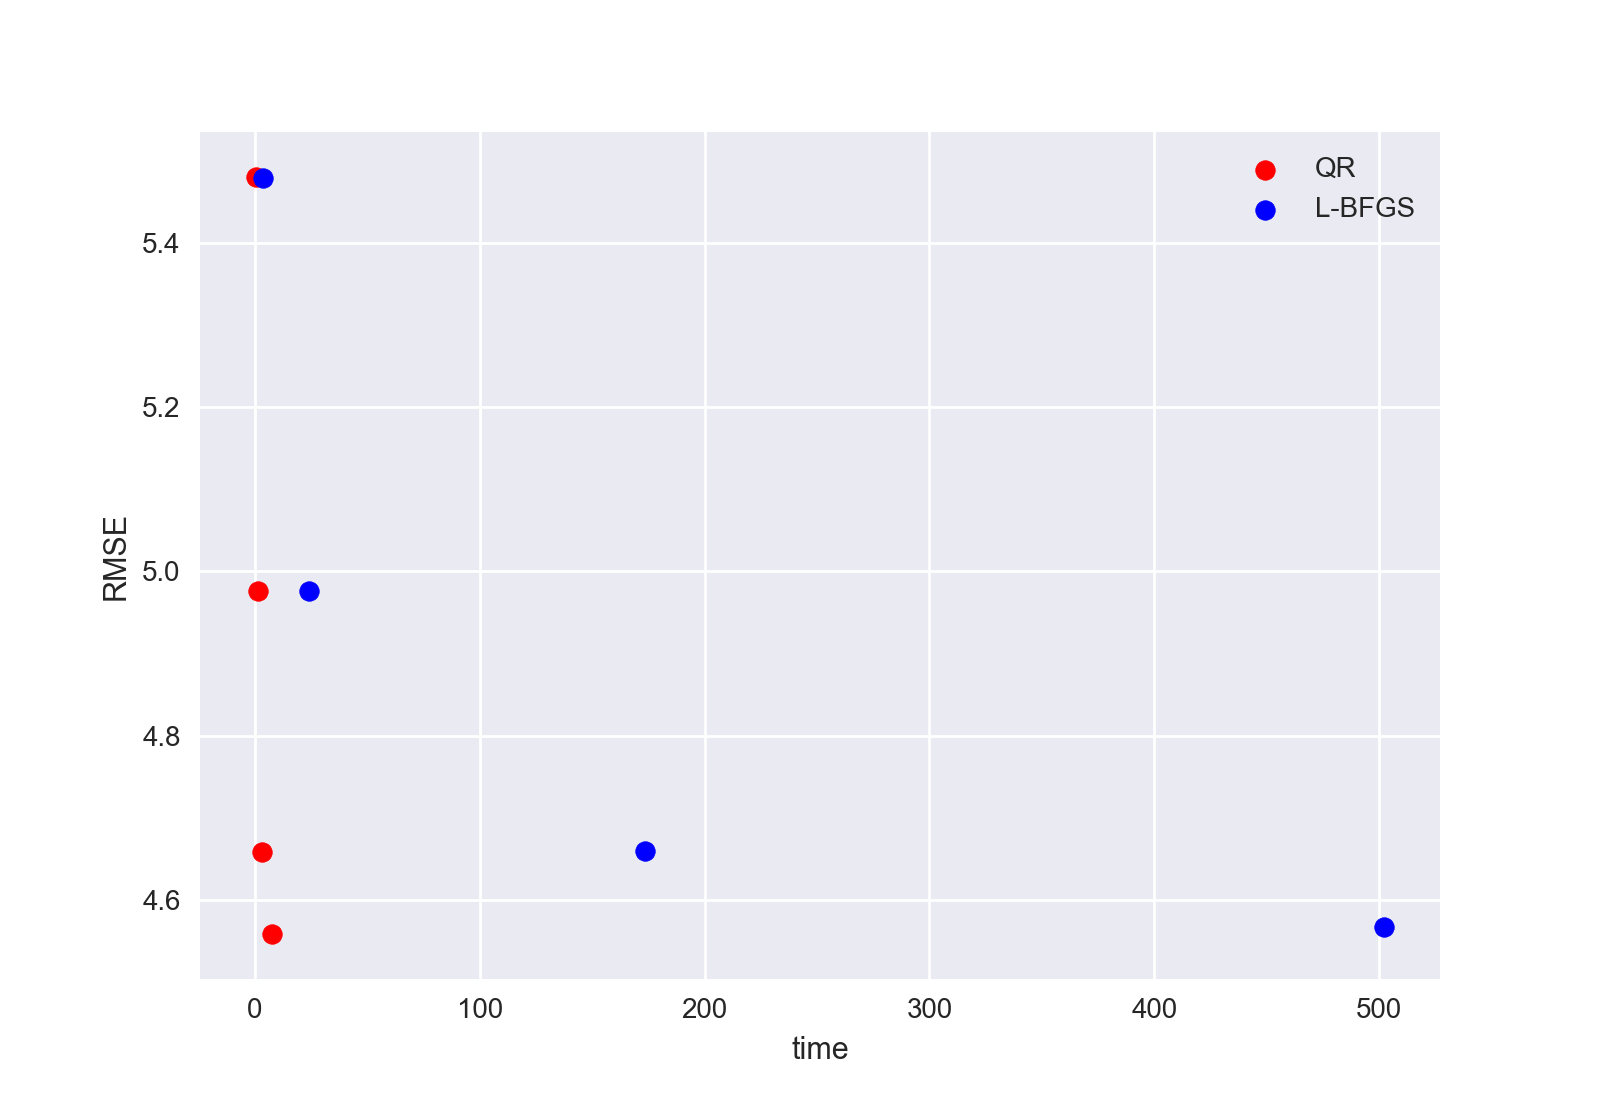
\includegraphics[scale=0.5]{1.png}
\end{center}


\end{document}
